\documentclass[12pt]{article}

\usepackage[utf8]{inputenc}
\usepackage[T1]{fontenc}
\usepackage[polish,provide=*]{babel}
\usepackage{lmodern}
\usepackage{amsmath}
\usepackage{latexsym,amsfonts,amssymb,amsthm,amsmath}
\usepackage{enumitem}
\usepackage{hyperref}
\usepackage{float}
\usepackage{graphicx}
\usepackage{subcaption}
\usepackage{booktabs}
\graphicspath{{./images/}}

\setlength{\parindent}{0in}
\setlength{\oddsidemargin}{0in}
\setlength{\textwidth}{6.5in}
\setlength{\textheight}{8.8in}
\setlength{\topmargin}{0in}
\setlength{\headheight}{18pt}

\title{Pomiar Zawartości Radonu w Powietrzu}
\author{Kacper Kłos}

\begin{document}

\maketitle

W niniejszym raporcie wyznaczyliśmy zawartość radonu na podstawie produktów jego rozpadu oraz zbadaliśmy zależność promieniowania od odległości. Najpierw umieszczaliśmy próbkę toru-232 nad scyntylatorem i rejestrowaliśmy jego odczyty podczas 2-minutowych interwałów, po czym zwiększaliśmy dystans między próbką a detektorem. Na podstawie dopasowania danych w skali log–log uzyskaliśmy, że liczba zarejestrowanych cząstek jest proporcjonalna do odwrotności odległości: \(N \propto 1/r\). Później, przy pomocy paru pomiarów promieniowania tła oszacowaliśmy dla jakiego dystansu odbierane promieniowanie nie pochodziło od toru. Na podstawie tych danych wyznaczyliśmy zakres energi cząstek alfa na \(E \in (3{,}6 4{,}5) MeV\).

Następnie wykorzystaliśmy metodę Markova, służącą do wyznaczania zawartości polonu w powietrzu, który powstaje w wyniku rozpadu radonu. Pomiar polegał na serii cykli pompowania powietrza przez filtr (ze zliczaniem objętości przepływającego gazu), a następnie dwóch pomiarach promieniowania rejestrowanego z tego filtra. Uzyskane wyniki wskazują, że koncentracja radonu w powietrzu: \((25 \pm 11)\,\mathrm{Bq\,m^{-3}}\) występuje nad stertą skał, 

\((9 \pm 6)\,\mathrm{Bq\,m^{-3}}\) w korytarzu przylegającym do pomieszczenia, w którym prowadzono pomiary, oraz \((10 \pm 9)\,\mathrm{Bq\,m^{-3}}\) w próbkach świeżego powietrza z zewnątrz.


\newpage

\section{Wstęp}
W niniejszym raporcie przedstawiamy zbadamy zawartości radonu w powietrzu pochodzącym z różnych otoczeń. Dodatkowo analizujemy, jak zmienia się zarejestrowane promieniowanie w funkcji odległości źródła od detektora cząstek. Przy pomocy tej zależności spróbujemy oszacować ile wynosi energia emitowanych cząstek.

\section{Podstawy Teoretyczne}
W naszych rozważaniach korzystamy głównie z prawa rozpadu promieniotwórczego, zgodnie z którym liczba jąder izotopu (np. radonu lub produktów jego rozpadu) maleje w czasie w tempie proporcjonalnym do bieżącej liczby jąder:
\[
\frac{dN(t)}{dt} \;=\; -\,\lambda\,N(t),
\]
gdzie \(\lambda\) jest dodatnią stałą rozpadu zależną od danego izotopu. Rozwiązaniem tego równania jest:
\begin{equation}
	N(t) \;=\; N(0)\,e^{-\lambda\,t}.
	\label{eq:decay}
\end{equation}

\section{Układ Doświadczalny}
Zarówno do pomiarów zależności natężenia promieniowania od odległości, jak i do określania zawartości radonu w powietrzu, wykorzystaliśmy ten sam detektor cząstek (jego dokładniejszy opis można znaleźć w \cite{skrypt}), który liczy rozpad w danym przedziale czasowym.

\subsection{Pomiar zależności od odległości}
Schemat układu przedstawiono na rys. \ref{fig:diagram}. Próbkę promieniotwórczego toru-232 umieszczano na regulowanym stojaku nad detektorem, a następnie zmieniano odległość między próbką a detektorem i mierzono liczbę zarejestrowanych rozpadów w ustalonym czasie (2 minuty).
Potem wykonaliśmy jeszcze parę pomiarów promienioawnia tła, aby oszacować przy jakiej odległości cząstki alfa nie docierają do detektora. Te dane pomogą nam oszacować energię emitowanego promieniowania.

\begin{figure}[H]
	\centering
	\includegraphics[scale=1]{układ}
	\caption{Układ pomiarowy do badania zależności promieniowania od odległości: 1 – miernik promieniowania, 2 – stojak z miarką, 3 – źródło promieniotwórcze.}
	\label{fig:diagram}
\end{figure}

\subsection{Pomiar zawartości radonu w powietrzu (metoda Markova)}
Do określania ilości polonu-218 (pochodnej radonu-222) w badanym powietrzu zastosowaliśmy metodę Markova \cite{equation}. Mierzone powietrze było przepompowywane przez filtr (na którym osadzały się produkty rozpadu), a później wykonywano dwa pomiary aktywności filtra, kładąc go bezpośrednio na detektor (rys. \ref{fig:diagram}), w ściśle określonych odstępach czasowych. Schemat cyklu to:
\begin{itemize}
	\item 5 minut – pompowanie powietrza przez filtr,
	\item 1 minuta – przerwa,
	\item 3 minuty – pierwszy pomiar aktywności filtra,
	\item 3 minuty – przerwa,
	\item 3 minuty – drugi pomiar aktywności filtra.
\end{itemize}
Graficzne przedstawienie cyklu widnieje na rys. \ref{fig:cycle}. Podczas pompowania monitorowano całkowitą objętość powietrza \(\nu\) za pomocą gazomierzu, a pomiary promieniowania przeprowadzono umieszczając filtr bezpośrednio nad detektorem.

\begin{figure}[H]
	\centering
	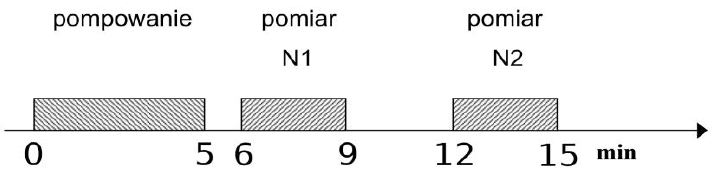
\includegraphics[scale=0.7]{cycle}
	\caption{Schemat cyklu pomiarowego (źródło: \cite{skrypt}).}
	\label{fig:cycle}
\end{figure}

Poprzez prostą analizę z urzyciem wzoru \eqref{eq:decay} otrzymana koncentracja polonu (co za tym idzie radonu) w powietrzu \(C_A\) wyraża się w postaci:
\[
    C_A \;=\; \frac{7{,}3 \times 10^{-5}\,\bigl(N_1 - N_2\bigr)}{\epsilon\,\nu\,\eta},
\]
gdzie \(N_1\) i \(N_2\) są zarejestrowanymi rozpadami w pierwszym i drugim okresie pomiarowym, \(\nu\) to objętość powietrza przepompowanego przez filtr w danym czasie, \(\epsilon\) oznacza wydajność rejestracji cząstek przez detektor, a \(\eta\approx 1\) jest efektywnością zatrzymywania produktów rozpadu na filtrze.  

W naszej analizie przyjęliśmy \(\eta=1\) oraz \(\epsilon \approx 0{,}0875\). Kulczowe założenia jakie poczyniliśmy to że promieniowanie roznosi się po sferze, zatem tylko \(50\%\) kieruje się w strone detektora, przy czym tylko \(45\%\) do niego dociera, a zostaje wykrytych jedynie $35\%$ cząstek.
Nasze oszacowanie opieramy na publikacjach \cite{scynt,alpha_range} i daje wspomniany wynik \(\epsilon \approx 0{,}0875\). Skutkiem tych oszacowań jest uproszczony wzór:
\begin{equation}
    C_A \;=\; \frac{83{,}43 \times 10^{-5}\,\bigl(N_1 - N_2\bigr)}{\nu}.
    \label{eq:markov}
\end{equation}

\section{Wyniki Pomiarów}

\subsection{Zależność promieniowania od odległości}
W pierwszej serii umieściliśmy próbkę toru nad detektorem (rys.~\ref{fig:diagram}) i mierzyliśmy liczbę zarejestrowanych rozpadów (w ciągu 120~s) przy różnych odległościach \(d\). Wyniki przedstawia tab.~\ref{tab:distance_measurments}.

\begin{table}[H]
	\centering
	\begin{tabular}{c|c|c}
		\toprule
        Nr & $N$ [Bq] & $d\,[\mathrm{cm}]$ \\
		\midrule
		1 & 36 & 1 \\
		2 & 22 & 2 \\
		3 & 12 & 3 \\
		4 & 10 & 4 \\
		5 & 6  & 5 \\
		\bottomrule
	\end{tabular}
	\caption{Pomiar natężenia promieniowania $N$ (liczba zliczeń w 120\,s) w funkcji odległości $d$ próbki od detektora.}
	\label{tab:distance_measurments}
\end{table}

Niepewność statystyczną zarejestrowanej liczby rozpadów szacujemy jako \(u(N)=\sqrt{N}\), a błąd odległości ustalamy na połowę podziałki \(\delta d=0{,}05\,\mathrm{cm}\). Zależność \(N(d)\) pokazuje rys.~\ref{fig:distance}.

\begin{figure}[H]
	\centering
	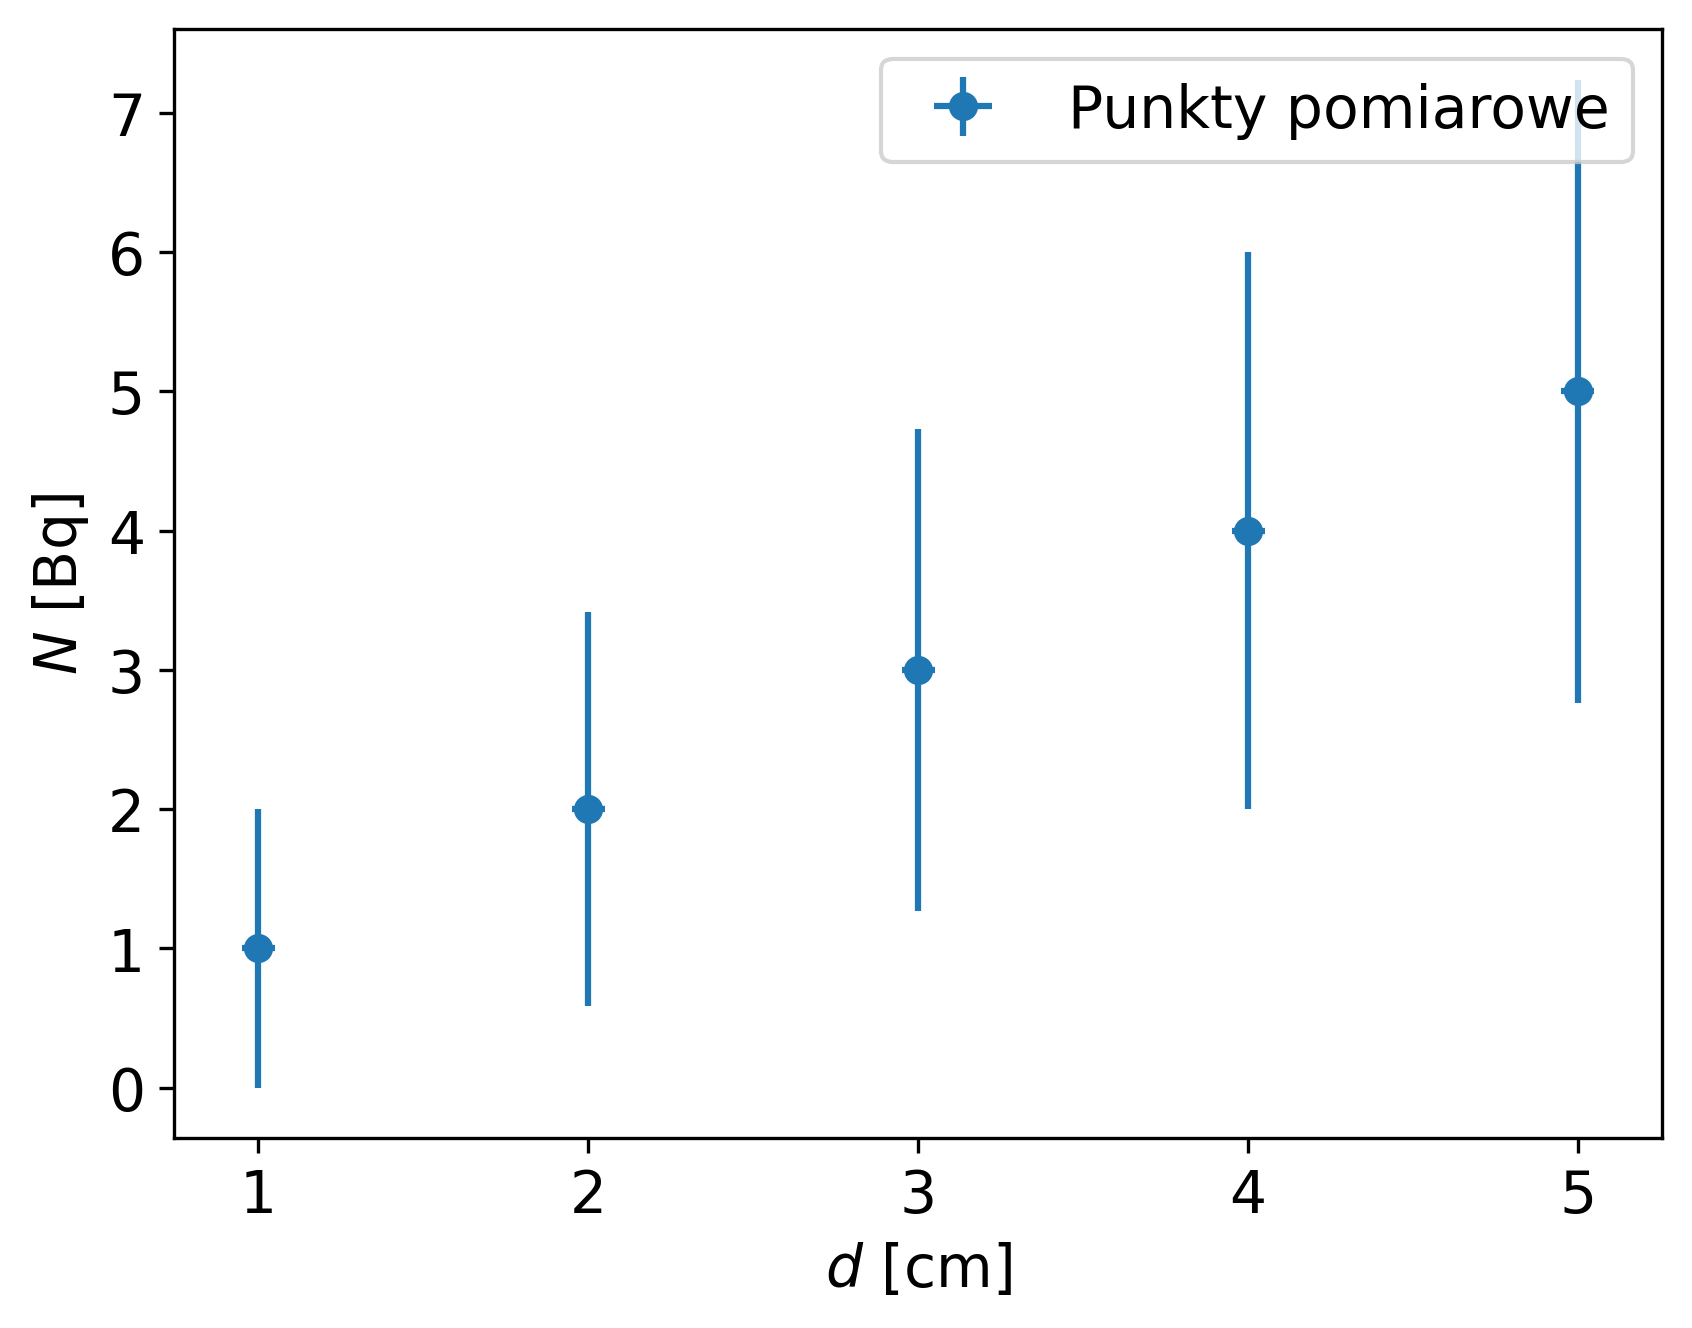
\includegraphics[scale=0.7]{distance}
	\caption{Zależność zarejestrowanych rozpadów $N$ od odległości $d$.}
	\label{fig:distance}
\end{figure}

Aby zbadać typową formę prawa potęgowego, przedstawiamy dane w skali log–log (rys.~\ref{fig:distance_log}) i dopasowujemy prostą: \(\log(N)=a\,\log(d)+b\).

\begin{figure}[H]
	\centering
	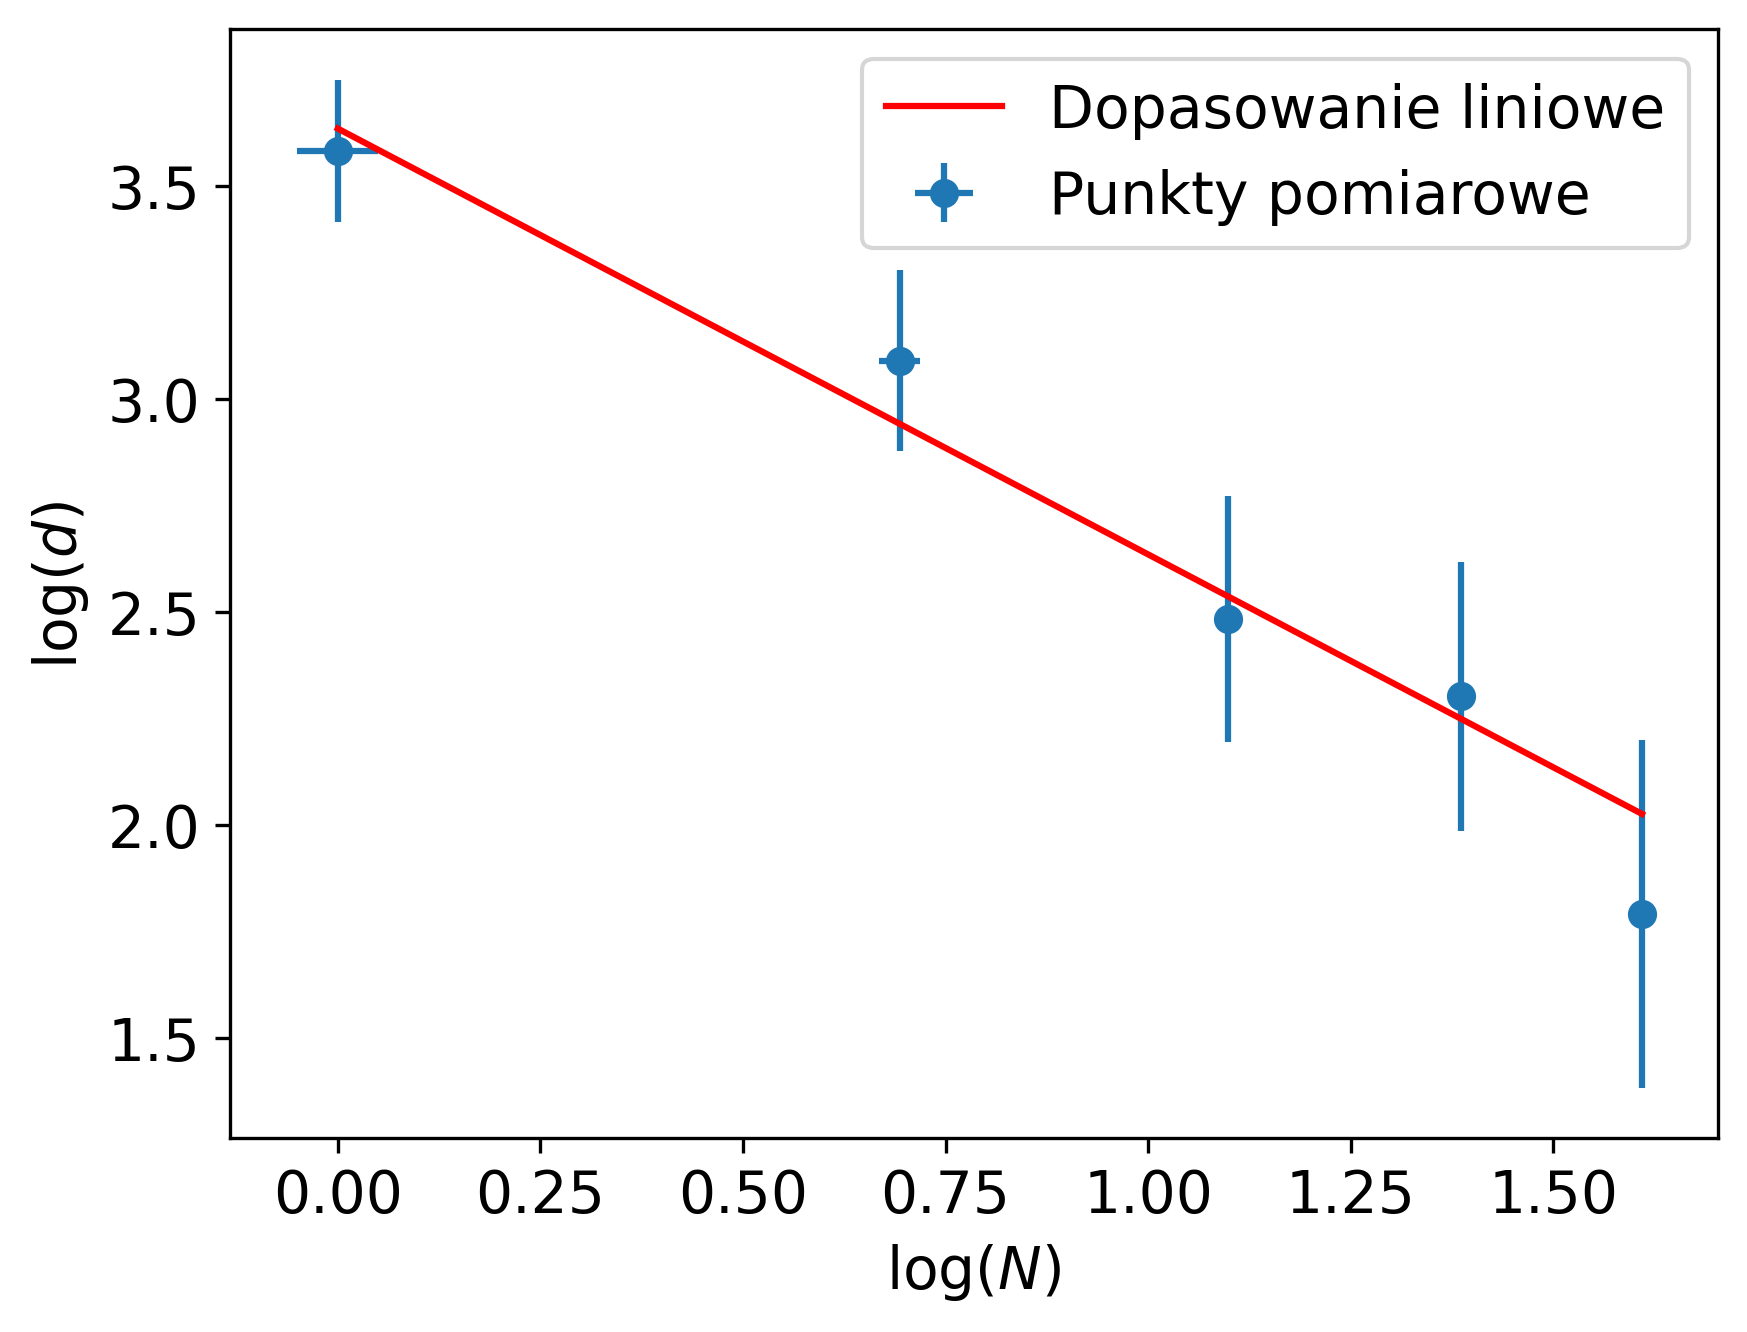
\includegraphics[scale=0.7]{distance_log}
	\caption{Wykres zależności $\log(N)$ od $\log(d)$.}
	\label{fig:distance_log}
\end{figure}

Dopasowanie dało:
\[
	a = -1{,}0 \pm 0{,}1, 
	\quad
	b = 3{,}6 \pm 0{,}1,
\]
co odpowiada zależności \(N \propto 1/d\). Warto jednak zaznaczyć, że w idealnym przypadku cząstki powinny rozchodzić się sferycznie (\(1/r^2\)) i maleć z powodu interakcji z powietrzem. Jednak uwzględniając duże błędy pomiarowe trudno jest dokładnie oszacować zależność.

Na podstawie pomiarów z tabeli~\ref{tab:background} w której widoczne są pomiary promieniowania tła dla 3 serii trwających 1 minutę możemy starać się oszacować energię emitowanych poprzez tor-232 cząstek alfa.
\begin{table}[H]
	\centering
	\begin{tabular}{c|c}
		\toprule
        Nr & $N_{\text{tło}}$ [Bq]\\
		\midrule
		1 & 3 \\
		2 & 2 \\
		3 & 2 \\
		\bottomrule
	\end{tabular}
	\caption{Pomiary zarejestrowanych cząstek \(N\) pochodzących od promieniowania tła w interwale 1 minuty.}
	\label{tab:background}
\end{table}

Widzimy że dla przedziału 1 minutowego pomiary mieszczą się w przedziale \(N_{tło_1} \in [2, 3]\). Na podstawie tego możemy wyznaczyć zakres ile cząstek takich interakcji powinno zajść w interwale 2 minutowym (2x większym od badanego).
Otrzymamy wtedy przedział \(N_{tło_2} \in [3,7]\) poszerzony o błąd pomiarowy będący w okolicach \(u(N_{tło_2}) = 1\).
Jedyna wartośc z danych dla pomiaru odległości (tab.~\ref{tab:distance_measurments}) która wpada w ten przedział to ostatni pomiar w którym otrzymaliśmy \(N = 6\) [Bq] dla dystansu \(d = 5\) cm. 
Także możemy wnioskować że zasięg cząstek alfa emitowanych przez tor-232 mieści się w przedziale (4cm, 5cm). Przy pomocy tabeli zależności zasięgu cząstek alfa od ich energi \cite{skrypt} możemy wyznaczyć przedział energetyczny cząstek alfa.
Na podstawie tych danych wyznaczamy przedział energii cząstek na \(E \in (3{,}6 4{,}5) MeV\).

\subsection{Koncentracja radonu (metoda Markova)}
Kolejno wykonaliśmy cykl opisany na rys.~\ref{fig:cycle} w trzech różnych miejscach: 
\begin{enumerate}[noitemsep]
	\item nad stertą kamieni (starsze próbki skalne),  
	\item w korytarzu tuż przed pomieszczeniem,  
	\item na zewnątrz (powietrze czerpane przez okno).
\end{enumerate}

W tab.~\ref{tab:density_measurments} zestawiono: $N_1$, $N_2$ – rozpad w dwóch pomiarach po cyklu pompowania powietrza, a także objętości powietrza przed i po pomiarze (\(V_{\text{przed}}\), \(V_{\text{po}}\)). Przyjmujemy błąd \(\sqrt{N_i}\) dla zarejestrowanych rozpadów, \(\delta V=0{,}01\,\mathrm{m^3}\) dla objętości oraz \(\delta t = 1s\).
Błąd na objętość (\(\delta V\)) oraz czas (\(\delta t\)) są znacznie poniżej \(1\%\), dlatego pozwalmy sobie go zignorować w dalszej części, skupiając się na błędzie pochodzącym ilości zarejestrowanych rozpadów.

\begin{table}[H]
	\centering
	\begin{tabular}{c|cc|cc}
		\toprule
		Środowisko & $N_1$ & $N_2$ & $V_{\text{przed}}\,[\mathrm{m^3}]$ & $V_{\text{po}}\,[\mathrm{m^3}]$ \\
		\midrule
		Kamienie & 132 & 95 & 2479{,}45 & 2483{,}13 \\
		Korytarz & 49  & 35 & 2483{,}13 & 2486{,}95 \\
		Podwórze & 91  & 76 & 2486{,}95 & 2490{,}87 \\
		\bottomrule
	\end{tabular}
	\caption{Rozpady w pierwszym ($N_1$) i drugim ($N_2$) okresie pomiarowym oraz objętość powietrza przed i po pompowaniu (metoda Markova).}
	\label{tab:density_measurments}
\end{table}

Całkowita objętość przepompowanego powietrza \(\nu\) stanowi różnicę \(\nu=\frac{V_{\text{po}}-V_{\text{przed}}}{300s}\). Przy założeniach opisanych w \ref{eq:markov} obliczamy koncentrację radonu \(C_A\). 

Błąd \(u(C_A)\) wynika głównie z niepewności \(\sqrt{N_1 + N_2}\), co prowadzi do:
\[
	u(C_A) \;=\; \frac{83{,}43 \times 10^{-5}\,\sqrt{N_1 + N_2}}{\nu}.
\]

Wyniki podsumowano w tab.~\ref{tab:concentration_results}.

\begin{table}[H]
	\centering
	\begin{tabular}{c|cc}
		\toprule
		Środowisko & $C_A\,[\mathrm{Bq\,m^{-3}}]$ & $u(C_A)\,[\mathrm{Bq\,m^{-3}}]$ \\
		\midrule
		Kamienie  & 25 & 11 \\
		Korytarz  & 9  & 6  \\
		Podwórze  & 10 & 9  \\
		\bottomrule
	\end{tabular}
	\caption{Wyniki wyznaczonego stężenia radonu w powietrzu metodą Markova, wraz z niepewnościami.}
	\label{tab:concentration_results}
\end{table}

\section{Podsumowanie}
W ramach przeprowadzonych badań wyznaczyliśmy zależność liczby zarejestrowanych rozpadów od odległości próbki toru-232 od detektora. Analiza w skali log–log zasugerowała zależność zbliżoną do \(1/d\), co odbiega od oczekiwanego wyniku. Jest to spowodowane ogromnymi niepewnościami w pomiarze rozpadów.
Także udało nam się oszacować przedział w jakim powinny znajdować się emitowane przez tor cząstki alfa \(E \in (3{,}6 4{,}5) MeV\). Jakość naszego oszacowania możemy określić na podstawie tabeli \cite{alpha_energy} z której odczytujemy że faktyczna energia wynosi \(E = 4{,}08 MeV\), co mieści się w wyznaczonym przedziale.

Następnie, stosując metodę Markova, oszacowaliśmy koncentrację radonu-222 (poprzez pomiar polonu-218) w powietrzu: 
\[
C_{A,\text{kamienie}}=(25 \pm 11)\,\mathrm{Bq\,m^{-3}}, 
\quad
C_{A,\text{korytarz}}=(9 \pm 6)\,\mathrm{Bq\,m^{-3}}, 
\quad
C_{A,\text{podwórze}}=(10 \pm 9)\,\mathrm{Bq\,m^{-3}}.
\]
Otrzymane wartości wskazują nieznacznie podwyższoną zawartość radonu przy stercie kamieni w porównaniu z korytarzem i otoczeniem zewnętrznym, co może być związane z większą obecnością minerałów zawierających tor czy uran. 

Z literatury \cite{concentration} wiadomo, że stężenia radonu w warunkach naturalnych mogą się znacznie różnić w zależności od geologii i wentylacji pomieszczeń. Nasze wyniki, choć obarczone znacznymi błędami (m.in. ze względu na ograniczoną wydajność detektora i przybliżenia co do zatrzymywania cząstek na filtrze), pokazują jednak pewną różnicę między miejscami z potencjalnie wyższym uwalnianiem radonu (skały) a miejscami mniej nim zanieczyszczonymi.

\newpage

\begin{thebibliography}{5}

	\bibitem{skrypt}
	\emph{Pomiar Zawartości Radonu w Powietrzu}, Uniwersytet Warszawski.

	\bibitem{equation}
	K.P. Markov, N.W. Rijabov, K.N. Stas, \emph{Atomnaja Energia 12}.

	\bibitem{scynt}
	\url{https://scintacor.com/wp-content/uploads/2021/09/Comparisons-of-new-simple-methods-in-fabricating-ZnS-Ag-scintillatiors-for-detecting-alpha-particles.pdf},
	\emph{Comparison of New Simple Methods in Fabricating ZnS(Ag) Scintillators for Detecting Alpha Particles}, 
	S. K. Lee, S. Y. Kang, D. Y. Jang et al.

	\bibitem{alpha_range}
	\url{https://www.rad-proceedings.org/papers/RadProc.2018.25.pdf},
	M. Y. A. Mostafa, M. V. Zhukovsky, \emph{Alpha Self-Absorption Evaluation in Radiometric Filter Material for the Natural Range of Alpha Energy (5–9 MeV)}.

	\bibitem{concentration}
	L. Dobrzyński i E. Droste, \emph{Promieniotwórczość a życie: problem ryzyka związanego z promieniowaniem jonizującym}, Raport Nr 12, Dział Szkolenia IPJ, Warszawa 1999.

    \bibitem{alpha_energy}
    \url{https://people.physics.anu.edu.au/~ecs103/chart/}, tablica nuklidów.

\end{thebibliography}

\end{document}
